\documentclass[../specific-algorithms.tex]{subfiles}
\begin{document}
In this chapter, we mainly discuss about the array based questions. We first categorize these problems into different type, and then each type can usually be solved and optimized with nearly the best efficiency. 

Here array means one dimension list. For array problems, math will play an important role here. The rules are as follows:
\begin{itemize}
    \item Subarray: using dynamic programming based algorithm to make brute force $O(n^3)$ to $O(n)$. Two pointers for the increasing subarray. Prefix sum, or kadane's algorithm plus sometimes with the hashmap, or two pointers (three pointers) for the maximum subarray. 
    \item Subsequence: using dynamic programming based algorithm to make brute force $O(2^n)$ to $O(n^2)$, which corresponds to the seqence type of dynamic programming. 
    \item Duplicates: 217, 26, 27, 219, 287, 442;
    \item Intersections of Two Arrays: 
\end{itemize}

Before we get into solving each type of problems, we first introduce the algorithms we will needed in this Chapter, including two pointers (three pointers or sliding window), prefix sum, kadane's algorithm. Kadane's algorithm can be explained with sequence type of dynamic programming. 

    % Easy problems: Duplicates:  Intersection: 349. Intersection of Two Arrays; Consecutive: 485. Max Consecutive Ones
    % Maximum/Minimum subarray: 718, 53. Maximum Subarray, 325. Maximum Size Subarray Sum Equals k. 209. Minimum Size Subarray Sum Solutions: divide and conquer, special sum and hashtable, two pointers (sliding window) for minimum
    % Sum of K numbers of elements: Target, return either the index or the elements(might need to avoid repetition). (2/3/4 sums)
    % Partition a list into K equal part: DP
    
After this chapter, we need to learn the step to solve these problems:
\begin{enumerate}
    \item Analyze the problem and categorize it.  To know the naive solution's time complexity can help us identify it.
    \item If we can not find what type it is, let us see if we can \textit{convert}. If not, we can try to identify a simple version of this problem, and then upgrade the simple solution to the more complex one. 
    \item Solve the problem with the algorithms we taught in this chapter.
    \item Try to see if there is any more solutions. 
    

    % \textit{Note: If the problem is complex, trying to see the simple version, and then upgrade the simple version to a complex one. e.g. (487. Max Consecutive Ones II, 485. Max Consecutive Ones)}
    \item Check the special case. (Usually very important for this type of problems)
\end{enumerate}
% Including two pointers both from the start, or two pointers one is from the beginning and the other is from the end. Also, the sliding window, and the flexible sliding windows, also find the cycle algorithm. 
%%%%%%%%%%%%%%%%%%%%%%%%%%%%%%%%%%%%%%%%%%%%%%%%%%%%%%%%%%%%%%%%%%%%%%%%%%%
%%%%% Algorithms
%%%%%%%%%%%%%%%%%%%%%%%%%%%%%%%%%%%%%%%%%%%%%%%%%%%%%%%%%%%%%%%%%%%%%%%%%%%
\section{Algorithms}
%%%%%%%%%%%%%%%%%%%%%%%%%%%%%%%%%%%%%%%%%%%%%%%%%%%%%%%%%%%%%%%%%%%%%%%%%%%
%%%%% Two Pointers
%%%%%%%%%%%%%%%%%%%%%%%%%%%%%%%%%%%%%%%%%%%%%%%%%%%%%%%%%%%%%%%%%%%%%%%%%%%
\subsection{Pointers and Sliding Window Algorithm}
T1: If you see in the problem that you can do comparison and it is always one type of satisfactory element is in ahead of the other, this could be resolved by two pointers (slower and faster). Note: when the while loop stops, is there operations you need?

Two pointers or three pointers are the most possible. \textit{Two pointers or three pointers is a superset of the sliding window algorithm, prefix sum too.} It can lower the complexity by one power level of n. 

\subsubsection{Two Pointers Sliding Window for Array}
674. Longest Continuous Increasing Subsequence
\begin{lstlisting}
Given an unsorted array of integers, find the length of longest continuous increasing subsequence (subarray).

Example 1:
Input: [1,3,5,4,7]
Output: 3
Explanation: The longest continuous increasing subsequence is [1,3,5], its length is 3. 
Even though [1,3,5,7] is also an increasing subsequence, it's not a continuous one where 5 and 7 are separated by 4.

Example 2:
Input: [2,2,2,2,2]
Output: 1
Explanation: The longest continuous increasing subsequence is [2], its length is 1.
\textit{Note: Length of the array will not exceed 10,000.}
\end{lstlisting}
Solution: The description of this problem should use ''subarray" instead of the ''subsequence".  The brute force solution is like any subarray problem $O(n^3)$. For embedded for loops to enumerate the subarray, and another $O(n)$ to check if it is strictly increasing.  Using two pointers, we can get $O(n)$ time complexity. We put two pointers: one $i$ located at the first element of the nums, second $j$ at the second element. We specifically restrict the subarray from $i$ to $j$ to be increasing, if this is violated, we reset the starting point of the subarray from the violated place.  
\begin{lstlisting}[language = Python]
class Solution:
    def findLengthOfLCIS(self, nums):
        """
        :type nums: List[int]
        :rtype: int
        """
        if not nums:
            return 0
        if len(nums)==1:
            return 1
        i,j = 0,0
        max_length = 0
        while j < len(nums):
            j += 1 #slide the window
            max_length = max(max_length, j-i)
            # when condition violated, reset the window
            if j<len(nums) and nums[j-1]>=nums[j]:
                i = j
                         
        return max_length
\end{lstlisting}

\subsubsection{Three Pointers Sliding  Window for Array}
Sometimes, by manipulating two pointers are not enough for us to get the final solution. 

930. Binary Subarrays With Sum
    \begin{lstlisting}
    In an array A of 0s and 1s, how many non-empty subarrays have sum S?
Example 1:

Input: A = [1,0,1,0,1], S = 2
Output: 4
Explanation: 
The 4 subarrays are bolded below:
[1,0,1,0,1]
[1,0,1,0,1]
[1,0,1,0,1]
[1,0,1,0,1]
Note:

    A.length <= 30000
    0 <= S <= A.length
    A[i] is either 0 or 1.
\end{lstlisting}
For example in the following problem, if we want to use two pointers to solve the problem, we would find we miss the case; like in the example $1, 0, 1, 0, 1$, when $j = 5$, $i = 1$, the sum is $2$, but the algorithm would miss the case of $i = 2$, which has the same sum value.
 
To solve this problem, we keep another index $i_hi$, in addition to the moving rule of $i$, it also moves if the sum is satisfied and that value is $0$. This is actually a Three pointer algorithm, it is also a mutant sliding window algorithm. 
\begin{lstlisting}[language=Python]
class Solution:
    def numSubarraysWithSum(self, A, S):
        i_lo, i_hi, j = 0, 0, 0 #i_lo <= j
        sum_window = 0
        ans = 0
        while j < len(A):

            sum_window += A[j]
                                     
            while i_lo < j and sum_window > S:
                sum_window -= A[i_lo]
                i_lo += 1
            # up till here, it is standard sliding window
            
            # now set the extra pointer at the same location of the i_lo
            i_hi = i_lo
            while i_hi < j and sum_window == S and not A[i_hi]:
                i_hi += 1
            if sum_window == S:
                ans += i_hi - i_lo + 1
                            
            j += 1 #increase the pointer at last so that we do not need to check if j<len again

        return ans
\end{lstlisting}

\subsubsection{Sliding Window for String: Anagram or Exact Matching}

%%%%%%%%%%%%%%%%%%%%%%%%%%%%%%%%%%%%%%%%%%%%%%%%%%%%%%%%%%%%%%%%%%%%%%%%%%%
%%%%% Prefex Sum
%%%%%%%%%%%%%%%%%%%%%%%%%%%%%%%%%%%%%%%%%%%%%%%%%%%%%%%%%%%%%%%%%%%%%%%%%%%
\subsection{Prefix Sum and Kadane's Algorithm}
\label{part4_prefix_sum}
In this section, we put prefix sum and kadance algorithm together because they are highly correlated to each others. They represents different perspective to solve a similary problem: one best example is the maximum subarray problem. 
\subsubsection{Introduction to Prefix Sum}
In computer science, the prefix sum, cumulative sum, inclusive scan, or simply scan of a sequence of numbers x0, x1, x2, ... is a second sequence of numbers y0, y1, y2, ..., the sums of prefixes (running totals) of the input sequence:
\begin{lstlisting}
    y0 = x0
    y1 = x0 + x1
    y2 = x0 + x1+ x2
    ...
\end{lstlisting}

For instance, the prefix sums of the natural numbers are the triangular numbers:
\begin{lstlisting}
    input numbers 	 1 	 2 	 3 	 4 	 5 	 6 	...
    prefix sums 	 1 	 3 	 6 	10 	15 	21 	... 
\end{lstlisting}

Prefix sums are trivial to compute in sequential models of computation, by using the formula $y_i = y_{i-1} + x_i$ to compute each output value in sequence order. And the sum of subarray needed in this section can be computed with formula $S_{(i,j)} = y_j-y_i$. However, despite their ease of computation, prefix sums are a useful primitive in certain algorithms such as counting sort,[1] as introduced in Section 2.3 of [2] and they form the basis of the scan higher-order function in functional programming languages.

\subsubsection{Prefix Sum Solution for Maximum Subarray Problem}
For the maximum subarray problem, we have our answer to be $max(y_j - y_i) (j>i, j\in[0,n-1])$, which is equivalent to $max(y_j - min(y_i)(i<j)), j\in[0,n-1]$. We can solve the maximum subarray problem using prefix sum with linear $O(n)$ time, where using brute force is $O(n^3)$ and the divide and conquer is $O(nlgn)$. For example, given an array of $[-2, -3, 4, -1, -2, 1, 5, -3]$. We have the following results:
\begin{table}[!ht]
\centering
\noindent\captionof{table}{ Process of using prefix sum for the maximum subarray}
\label{tab: prefix_sum}
 \noindent \begin{tabular}{c rrrrrrrr}
  \hline\hline
%   & Count & Percentage/Total Problems & Percentage/Total Data Structure \\ \hline
Array  & $-2$& $-3$ & $4$& $-1$& $-2$& $1$& $5$& $3$\\
prefix sum   & $-2$& $-5$ & $-1$& $-2$& $-4$& $-3$& $2$& $1$ \\
Updated prefix sum &$-2$& $-3$& $4$& $3$& $1$& $2$ &$7$&$ 4$ \\
current max sum & $-2$& $-2$ & $4$& $4$& $4$& $4$& $7$& $7$\\ 
min prefix sum & $-2$& $-5$ & $-5$& $-5$& $-5$& $-5$& $-5$& $-5$\\ \hline
\end{tabular}
\end{table}
The coding:
\begin{lstlisting}[language = Python]

# or we can use import math, math.inf

# Function to compute maximum 
# subarray sum in linear time. 
def maximumSumSubarray(nums): 
    if not nums:
        return 0
    prefixSum = 0
    globalA = -sys.maxsize
    minSub = 0
    for i in range(len(nums)):
        prefixSum += nums[i]
        globalA = max(globalA, prefixSum-minSub)
        minSub = min(minSub, prefixSum)
    return globalA

# Driver Program 

# Test case 1 
arr1 = [ -2, -3, 4, -1, -2, 1, 5, -3 ] 
print(maximumSumSubarray(arr1)) 

# Test case 2 
arr2 = [ 4, -8, 9, -4, 1, -8, -1, 6 ] 
print(maximumSumSubarray(arr2)) 
\end{lstlisting}
As we can see, we did not need extra space to save the prefix sum, because each time we only use prefix sum at current index. 

\subsubsection{Kadane Algorithm Solution to Maximum Subarray Problem}
\textbf{Mutant of Prefix Sum:} Another easier perspective using dynamic programming for this problem because we found the key word ''Maximum" in the question which is problem that identified in the dynamic programming chapter. 
\begin{lstlisting}
dp: the maximum subarray result till index i, which includes the current element nums[i]. We need n+1 space due to using i-1.
Init: all 0
state transfer function: dp[i] = max(dp[i-1]+nums[i], nums[i]); because if for each element, we can either continue the previous subarray or start a new subarray. 
Result: max(dp)
\end{lstlisting}
However, to do space optimization, we only need to track the current maximum $dp$ and since $dp[i]$ is only related to $dp[i-1]$. For the last example, the newly updated prefix sum is $-2, -3, 4, 3, 1, 2, 7, 4$. The comparison result can be seen in Table~\ref{tab: prefix_sum}. 
\begin{lstlisting}[language=Python]
def maximumSumSubarray(arr): 
    if not arr:
        return 0
    dp = [0]*(len(arr)+1)
    #max_so_far = -sys.maxsize
    for i in range(len(arr)):
        dp[i+1] = max(dp[i]+arr[i], arr[i])
    return max(dp)
\end{lstlisting}

%%%%%%%%%%%%%%%%%%%%%%%%%%%%%%%%%%%%%%%%%%%%%%%%%%%%%%%%%%%%%%%%%%%%%%%%%%%
%%%%% Kadane Algorithm
%%%%%%%%%%%%%%%%%%%%%%%%%%%%%%%%%%%%%%%%%%%%%%%%%%%%%%%%%%%%%%%%%%%%%%%%%%%
Because we can still do space optimization to the above solution, we use one variable to replace the dp array, and we track the maximum dp in the for loop instead of obtaining the maximum value at the end. Also, if we rename the dp to max\_ending\_here and the max(dp) to max\_so\_far, the code is as follows:
\begin{lstlisting}[language=Python]
def maximumSumSubarray(arr, n): 
    if not arr:
        return 0
    max_ending_here = 0
    max_so_far = -sys.maxsize
    for i in range(len(arr)):
        max_ending_here = max(max_ending_here+arr[i], arr[i])
        max_so_far = max(max_so_far, max_ending_here)
    return max_so_far
\end{lstlisting}
This space-wise optimized dynamic programming solution to the maximum subarray problem is exactly the Kadane's algorithm.  Kadane's algorithm begins with a simple inductive question: if we know the maximum subarray sum ending at position $i$, what is the maximum subarray sum ending at position $i+1$? The answer turns out to be relatively straightforward: either the maximum subarray sum ending at position $i+1$ includes the maximum subarray sum ending at position $i$ as a prefix, or it doesn't. Thus, we can compute the maximum subarray sum ending at position $i$ for all positions $i$ by iterating once over the array. As we go, we simply keep track of the maximum sum we've ever seen. Thus, the problem can be solved with the following code, expressed here in Python:
\begin{lstlisting}[language = Python]
def max_subarray(A):
    max_ending_here = max_so_far = A[0]
    for x in A[1:]:
        max_ending_here = max(x, max_ending_here + x)
        max_so_far = max(max_so_far, max_ending_here)
    return max_so_far
\end{lstlisting}

The algorithm can also be easily modified to keep track of the starting and ending indices of the maximum subarray (when max\_so\_far changes) as well as the case where we want to allow zero-length subarrays (with implicit sum 0) if all elements are negative. For example: 

Now, let us see how we do maximum subarray with product operation instead of the sum. 

152. Maximum Product Subarray
\begin{lstlisting}
Given an integer array nums, find the contiguous subarray within an array (containing at least one number) which has the largest product.

Example 1:

Input: [2,3,-2,4]
Output: 6
Explanation: [2,3] has the largest product 6.

Example 2:

Input: [-2,0,-1]
Output: 0
Explanation: The result cannot be 2, because [-2,-1] is not a subarray.
\end{lstlisting}

Answer: For the product, the difference compared with sum is the max\_ending\_here is not necessarily computed from the previous value with current element; if the element is negative it might even become the smallest. So that we need to track another variable, the min\_ending\_here. Let use see the Python code which is a straightforward implementation of the product-modified kadane's algorithm. 
\begin{lstlisting}
from sys import maxsize
class Solution(object):
    def maxProduct(self, nums):
        """
        :type nums: List[int]
        :rtype: int
        """
        if not nums:
            return 0
        n = len(nums)
        max_so_far = nums[0]
        min_local, max_local = nums[0], nums[0]
        for i in range(1, n):
            a = min_local*nums[i]
            b = max_local*nums[i]
            max_local = max(nums[i], a, b)
            min_local = min(nums[i], a, b)
            max_so_far = max(max_so_far, max_local)
        return max_so_far
\end{lstlisting}





%%%%%%%%%%%%%%%%%%%%%%%%%%%%%%%%%%%%%%%%%%%%%%%%%%%%%%%%%%%%%%%%%%%%%%%%%%%
%%%%% rabbit and turtle to find circle or repeat number
%%%%%%%%%%%%%%%%%%%%%%%%%%%%%%%%%%%%%%%%%%%%%%%%%%%%%%%%%%%%%%%%%%%%%%%%%%%
\subsection{Floyd’s Cycle-Finding Algorithm}

Without this we detect cycle with the following code:
\begin{lstlisting}[language = Python]
def detectCycle(self, A):
        visited=set()       
        head=point=A
        while point:
            if point.val in visited:
                return point
            visited.add(point)
            point=point.next
        return None
\end{lstlisting}

Traverse linked list using two pointers. Move one pointer by one and other pointer by two. If these pointers meet at some node then there is a loop. If pointers do not meet then linked list doesn’t have loop. Once you detect a cycle, think about finding the starting point.
\begin{figure}[h!]
    \centering
    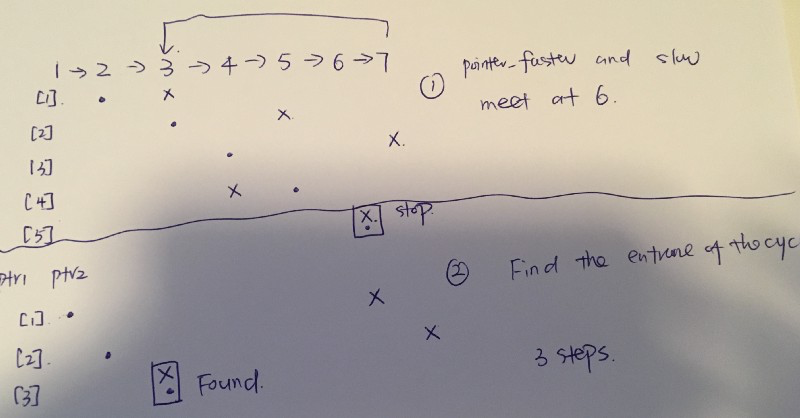
\includegraphics[width = 0.98\columnwidth]{fig/floyd.png}
    \caption{Example of floyd’s cycle finding}
    \label{fig:floyd}
\end{figure}

\begin{lstlisting}[language = Python]
def detectCycle(self, A):
        #find the "intersection" 
        p_f=p_s=A
        while (p_f and p_s and p_f.next):
            p_f = p_f.next.next
            p_s = p_s.next
            if p_f==p_s:
                break
        #Find the "entrance" to the cycle.
        ptr1 = A
        ptr2 = p_s;
        while ptr1 and ptr2:
            if ptr1!=ptr2:
                ptr1 = ptr1.next
                ptr2 = ptr2.next
            else:
                return ptr1
        return None
\end{lstlisting}

\subsection{Longest Common Subsequence}
Longest common substring is actually a sub-algorithm from the double sequence type Dynamic programming. 

Suppose we have string A and B, each with m and n chars. If we use brute force, then in A, there could be $M^2$ substring, and to locate these substring in B, we spend O(n) for each substring, which makes the total complexity to be $O(n*M^2)$. \textit{Note: it is the same if its two arrays.} But now, if we use the LCS method, the time and space complexity will be $O(n*m)$ . LCS is DP method that we can use bottom-up with memorization.
\begin{figure}[h]
    \centering
    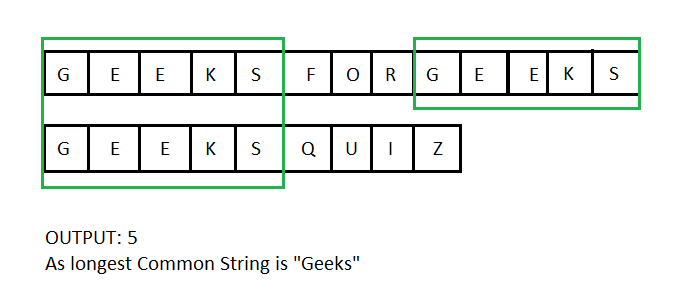
\includegraphics[width = 0.98\columnwidth]{fig/lcs.png}
    \caption{Longest common substring}
    \label{fig:lcs}
\end{figure}
\begin{lstlisting}[language = Python]
Pseudo-code of LCS
#init a[M+1][N+1] two dimensional matrix with [0]
a =[[0 for _ in xrange(N+1)] for _ in xrange(M+1)]
for i in [0,M):
    for j in [0,N):
        if A[i]==A[j]:
            a[i+1][j+1]=a[i][j]+1
            result = max(result,a[i+1][j+1])

        else:
            a[i+1][j+1] = 0
\end{lstlisting}
Although the algorithm is named with ''substring", however, they are equivalent the maximum intersection ''subarray".

718. Maximum Length of Repeated Subarray (Medium)
\begin{lstlisting}
Given two integer arrays A and B, return the maximum length of an subarray that appears in both arrays.

Example 1:

Input:
A: [1,2,3,2,1]
B: [3,2,1,4,7]
Output: 3
Explanation: 
The repeated subarray with maximum length is [3, 2, 1].

Note:

    1 <= len(A), len(B) <= 1000
    0 <= A[i], B[i] < 100
\end{lstlisting}
Using LCS the time complexity if $O(n*m)$.
\begin{lstlisting}[language = Python]
class Solution:
    def findLength(self, A, B):
        """
        :type A: List[int]
        :type B: List[int]
        :rtype: int
        """
        if not A or not B:
            return 0
        result = 0
        a =[[0 for _ in range(len(B)+1)] for _ in range(len(A)+1)]
        for i in range(len(A)):
            for j in range(len(B)):
                if A[i]==B[j]:
                    a[i+1][j+1] = a[i][j]+1
                    result = max(result, a[i+1][j+1])
                else:
                    a[i+1][j+1] = 0
        return result
\end{lstlisting}
% \subsection{Examples-Intersections}
% \begin{enumerate}
%     \item 

% \end{enumerate}


%%%%%%%%%%%%%%%%%%%%%%%%%%%%%%%%%%%%%%%%%%%%%%%%%%%%%%%%%%%%%%%%%%%%%%%%%%%
%%%%% Examples
%%%%%%%%%%%%%%%%%%%%%%%%%%%%%%%%%%%%%%%%%%%%%%%%%%%%%%%%%%%%%%%%%%%%%%%%%%%
\section{Different Type of Questions}
%%%%%%%%%%%%%%%%%%%%%%%%%%%%%%%%%%%%%%%%%%%%%%%%%%%%%%%%%%%%%%%%%%%%%%%%%%%
%%%%% Subarray
%%%%%%%%%%%%%%%%%%%%%%%%%%%%%%%%%%%%%%%%%%%%%%%%%%%%%%%%%%%%%%%%%%%%%%%%%%%
\subsection{Subarray (Easy) }
\textit{Note: For subarray the most important feature is contiguous. Here, we definitely will not use sorting.}



Given a single array, we would normally be asked to return either the maximum/minimum value, the maximum/minimum length, or the number of subarrays that has sum/product that \textit{satisfy a certain condition}. The condtion here decide the difficulty of these problems.

The questions can are classified into two categories: \textit{Absolute-conditioned Subarray} that $sum/product=K$ or \textit{Vague-conditioned subarray} that has these symbols that is not equal. 


% \begin{enumerate}
%     \item Maximum/minimum subarray with Sum or Product or a pattern; we use \textbf{math and prefix\_sum} or sometimes together with hashmap method to tackle. Also, sliding window can be used.
%     \item Minimum Subarray with Sum or Product or a pattern; \textbf{sliding window} can be used to get the minimum length of subarray. 
%     \item Find subarray that is increasing or decreasing ; \textbf{Two pointers or sliding window} can be used. 
% \end{enumerate}
With the proposed algorithms, the time complexity of subarray problems can be decreased from the brute force $O(n^3)$ to $O(n)$. The brute force is universal: two embedded for loops marked the start and end of the subarray to enumerate all the possible subarrays, and another $O(n)$ spent to compute the result needed (sum or product or check the pattern like increasing or decreasing). 

Using prefix sum or kadane's algorithm or hashmap sometimes if we have problems to solve it, a panacea is the Sliding Window Algorithm either with two or three pointers. 
%%%%%%%%%%%%%%%%%%%%%%%%%%%%%%%%%%%%%%%%%%%%%%%%%%%%%%%%%%%%%%%%%%%%%%%%%%%
%%%%% Maximum Subarray
%%%%%%%%%%%%%%%%%%%%%%%%%%%%%%%%%%%%%%%%%%%%%%%%%%%%%%%%%%%%%%%%%%%%%%%%%%%
\subsubsection{Absolute-conditioned Subarray}
For the maximum array, you are either asked to return: 
\begin{enumerate}
\item the maximum sum or product; \textit{solved using prefix sum or kadane's algorithm}
\item the maximum length of subarray with sum or product S equals to K; \textit{solved using prefix sum together with a hashmap saves previous prefix sum and its indices}
\item the maximum number of subarray with sum or product S (the total number of) equals to K; \textit{solved using prefix sum together with a hashmap saves previous prefix sum and its count}
\end{enumerate}

\paragraph{Maximum/Minimum sum or product}

53. Maximum Subarray

\begin{lstlisting}
Find the contiguous subarray within an array (containing at least one number) which has the largest sum.

For example, given the array [-2,1,-3,4,-1,2,1,-5,4],
 the contiguous subarray [4,-1,2,1] has the largest sum = 6.
\end{lstlisting}
Solution: Brute force is to use two for loops, first is the starting, second is the end, then we can get the maximum value. To optimize, we can use divide and conquer, $O(nlgn)$ vs brute force is $O(n^3)$ (two embedded for loops and n for computing the sum). The divide and conquer method was shown in that chapter. A more efficient algorithm is using pre\_sum. Please check Section~\ref{part4_prefix_sum} for the answer. 

Now what is the slinding window solution? The key step in sliding window is when to move the first pointer of the window (shrinking the window). The window must include current element j. For the maximum subarray, to increase the sum of the window, we need to abandon any previous elements if they have negative sum.
\begin{lstlisting}[language = Python]
from sys import maxsize
class Solution:
    def maxSubArray(self, nums):
        """
        :type nums: List[int]
        :rtype: int
        """
        if not nums:
            return 0
        i, j = 0, 0 #i<=j
        maxValue = -maxsize
        window_sum = 0
        while j < len(nums):
            window_sum += nums[j]
            j += 1
            maxValue = max(maxValue, window_sum)
            while i<j and window_sum < 0:
                window_sum -= nums[i]
                i += 1                           
        return maxValue
\end{lstlisting}

\paragraph{Maximum/Minimum length of subarray with sum or product S}
For this type of problem we need to track the length of it. 

% \begin{enumerate}
325. Maximum Size Subarray Sum Equals k

Given an array nums and a target value k, find the maximum length of a subarray that sums to k. If there isn’t one, return 0 instead.

Note:
 The sum of the entire nums array is guaranteed to fit within the 32-bit signed integer range.

\begin{lstlisting}
Example 1:
Given nums = [1, -1, 5, -2, 3], k = 3,
 return 4. (because the subarray [1, -1, 5, -2] sums to 3 and is the longest)

Example 2:
Given nums = [-2, -1, 2, 1], k = 1,
 return 2. (because the subarray [-1, 2] sums to 1 and is the longest)

Follow Up:
 Can you do it in O(n) time?
 \end{lstlisting}
Answer: the brute force solution of this problem is the same as the maximum subarray. The similarity here is we track the prefix sum $S_{(i,j)} = y_j - y_i$, if we only need to track a certain value of $S_{(i,j)}$, which is $k$. Because $y_i = y_j - k$ which is the current prefix sum minus the k. If we use a hashmap to save the set of prefix sum together with the first index of this value appears. We saved $(y_i, first\_index)$, so that $max\_len = max(idx-dict[y_j-k])$. 
% Solution: using prefix\_sum and hashmap, to just need to reformulate dict[sum\_i]. For this question, we need to get the maximum size of subarray, so dict[i] =min(idx), the earliest that the value appear. which means every time we just set the $dict[i]=current_index$, only if the key does'nt exist. dict[0] = -1. Here we have sum\_i, to check if there is a j in front of i that makes sum(j,i)=k, sum(j,i)=sum\_i-A Value in Dict = k, so the value need to be sum\_i-k, so that we need to check if it is in the dictionary.
\begin{lstlisting}[language = Python]
def maxSubArrayLen(self, nums, k):
        """
        :type nums: List[int]
        :type k: int
        :rtype: int
        """
        prefix_sum = 0
        dict = {0:-1} #this means for index -1, the sum is 0
        max_len = 0
        for idx,n in enumerate(nums):
            prefix_sum += n
            # save the set of prefix sum together with the first index of this value appears. 
            if prefix_sum not in dict: 
                dict[prefix_sum] = idx
            # track the maximum length so far
            if prefix_sum-k in dict:
                max_len=max(max_len, idx-dict[sum_i-k])
        return max_len
\end{lstlisting}

Another example that asks for pattern but can be converted or equivalent to the last problems:

525. Contiguous Array

Given a binary array, find the maximum length of a contiguous subarray with equal number of 0 and 1.

Example 1:
\begin{lstlisting}
Input: [0,1]
Output: 2
Explanation: [0, 1] is the longest contiguous subarray with equal number of 0 and 1.

Example 2:

Input: [0,1,0]
Output: 2
Explanation: [0, 1] (or [1, 0]) is a longest contiguous subarray with equal number of 0 and 1.

\textit{Note: The length of the given binary array will not exceed 50,000.}
\end{lstlisting}

Solution: the problem is similar to the maximum sum of array with sum==0, so 0=-1, 1==1. Here our $k=0$
\begin{lstlisting}[language = Python]
def findMaxLength(self, nums):
        """
        :type nums: List[int]
        :rtype: int
        """
        nums=[nums[i] if nums[i]==1 else -1 for i in range(len(nums))]
        
        max_len=0
        cur_sum=0
        mapp={0:-1}
        
        for idx,v in enumerate(nums):
            cur_sum+=v
            if cur_sum in mapp:
                max_len=max(max_len,idx-mapp[cur_sum])
            else:
                mapp[cur_sum]=idx    
        
        return max_len
\end{lstlisting}

%%%%%%%%%%%%%%%%%%%%%%%%%%%%%%%%%%%%%%%%%%%%%%%%%%%%%%%%%%%%%%%%%%%%%%%%%%%
%%%%% Maximum Subarray
%%%%%%%%%%%%%%%%%%%%%%%%%%%%%%%%%%%%%%%%%%%%%%%%%%%%%%%%%%%%%%%%%%%%%%%%%%%
\paragraph{The maximum number of subarray with sum or product S}

560. Subarray Sum Equals K
\begin{lstlisting}
Given an array of integers and an integer k, you need to find the total number of continuous subarrays whose sum equals to k.

Example 1:
Input:nums = [1,1,1], k = 2
Output: 2
\end{lstlisting}

Answer: The naive solution is we enumerate all possible subarray which is $n^2$, and then we compute and check its sum which is $O(n)$. So the total time complexity is  $O(n^3)$ time complexity. However, we can decrease it to $O(n^2)$ if we compute the sum of array in a different way: we first compute the sum till current index for each position, with equation $sum(i,j) = sum(0,j)-sum(0,i)$. However the OJ gave us LTE error. 
\begin{lstlisting}[language = Python]
def subarraySum(self, nums, k):
        """
        :type nums: List[int]
        :type k: int
        :rtype: int
        """
        ''' return the number of subarrays that equal to k'''
        count = 0
        sums = [0]*(len(nums)+1) # sum till current index
        for idx, v in enumerate(nums):
            sums[idx+1] = sums[idx]+v
        for i in range(len(nums)):
            for j in range(i, len(nums)):
                value = sums[j+1]-sums[i]
                count = count+1 if value==k else count
        return count
\end{lstlisting}

Solution 3: using prefix\_sum and hashmap, to just need to reformulate dict[sum\_i]. For this question, we need to get the total number of subsubarray, so $dict[i] = count$, which means every time we just set the dict[i]+=1. dict[0]=1
\begin{lstlisting}[language = Python]
import collections
class Solution(object):
    def subarraySum(self, nums, k):
        """
        :type nums: List[int]
        :type k: int
        :rtype: int
        """
        ''' return the number of subarrays that equal to k'''
        dict = collections.defaultdict(int) #the value is the number of the sum occurs
        dict[0]=1
        prefix_sum, count=0, 0
        for v in nums:
            prefix_sum += v
            count += dict[prefix_sum-k] # increase the counter of the appearing value k, default is 0
            dict[prefix_sum] += 1 # update the count of prefix sum, if it is first time, the default value is 0
        return count
\end{lstlisting}



%%%%%%%%%%%%%%%%%%%%%%%%%%%%%%%%%%%%%%%%%%%%%%%%%%%%%%%%%%%%%%%%%%%%%%%%%%%
%%%%% Vague-conditioned subarray
%%%%%%%%%%%%%%%%%%%%%%%%%%%%%%%%%%%%%%%%%%%%%%%%%%%%%%%%%%%%%%%%%%%%%%%%%%%
\subsubsection{Vague-conditioned subarray}
In this section, we would be asked to ask the same type of question comapred with the last section. The only difference is the condition. For example, in the following question, it is asked with subarray that with $sum >= s$. 

Because of the vague of the condition, a hashmap$+$prefix sum solution will on longer give us $O(n)$ liner time. The best we can do if the array is all positive number we can gain $O(nlgn)$ if it is combined with binary search. However, a carefully designed sliding window can still help us achieve linear time. 

\paragraph{All Positive Array}

If it is all positive array, it can still be easily solved with sliding window. For example: 

209. Minimum Size Subarray Sum
\begin{lstlisting}
Given an array of n positive integers and a positive integer s, find the minimal length of a contiguous subarray of which the sum >= s. If there isn't one, return 0 instead.
Example: 

Input: s = 7, nums = [2,3,1,2,4,3]
Output: 2
Explanation: the subarray [4,3] has the minimal length under the problem constraint.

Follow up:
If you have figured out the O(n) solution, try coding another solution of which the time complexity is O(n log n). 
\end{lstlisting}
For this problem, if we use prefix sum, we need to save the last index of the prefix sum compared with the maximum length problem. However, with this problem the condition is $sum >= s$, if we use a hashmap, we need to search through the hashmap with $key <= prefix_sum - s$. The time complexity would rise up to $O(n^2)$. We would receive LTE error.
\begin{lstlisting}[language = Python]
    def minSubArrayLen(self, s, nums):
        """
        :type s: int
        :type nums: List[int]
        :rtype: int
        """
        if not nums:
            return 0
        dict = collections.defaultdict(int)
        dict[0] = -1 # pre_sum 0 with index -1
        prefixSum = 0
        minLen = sys.maxsize
        for idx, n in enumerate(nums):
            prefixSum += n
            for key, value in dict.items():
                if key <= prefixSum - s: 
                    minLen = min(minLen, idx-value)
            dict[prefixSum] = idx #save the last index
        return minLen if 1<=minLen<=len(nums) else 0
\end{lstlisting}
Because if we use prefix sum and use brute force to enumerate the subarray we gain $O(n^2)$. In this problem because its all positive number, so the prefix sum array is increasing which means we can use binary search to find the largest value that is smaller than or equal to prefix sum - s.
\begin{lstlisting}[language = Python]
    def minSubArrayLen(self, s, nums):
        """
        :type s: int
        :type nums: List[int]
        :rtype: int
        """
        def bSearch(nums, i, j, target):
            while i < j:
                mid = (i+j) / 2
                if nums[mid] == target:
                    return mid
                elif nums[mid] < target:
                    i = mid + 1
                else:
                    j = mid - 1
            return i   
        
        if not nums:
            return 0
        rec = [0] * len(nums)
        rec[0] = nums[0]
        if rec[0] >= s:
            return 1
        minlen = len(nums)+1
        for i in range(1, len(nums)):
            rec[i] = rec[i-1] + nums[i]
            if rec[i] >= s:
                index = bSearch(rec, 0, i, rec[i] - s)
                if rec[index] > rec[i] - s:
                    index -= 1
                minlen = min(minlen, i - index)
        return minlen if minlen != len(nums)+1 else 0
\end{lstlisting}
While, using the sliding window, we are still capable of getting the complexity with $O(n)$. 
\begin{lstlisting}[language = Python]
    def minSubArrayLen(self, s, nums):
            """
            :type s: int
            :type nums: List[int]
            :rtype: int
            """
            i,j = 0,0
            preSum =0
            min_length = len(nums)+1
            while j < len(nums):          
                preSum += nums[j]
                j+=1
                #shrink the sliding window size
                while i < j and preSum >= s:
                    min_length = min(min_length, j-i)
                    preSum -= nums[i] #shrink
                    i += 1
            return min_length if min_length< len(nums)+1 else 0
\end{lstlisting}

713. Subarray Product Less Than K

\begin{lstlisting}
Your are given an array of positive integers nums.
Count and print the number of (contiguous) subarrays where the product of all the elements in the subarray is less than k.

Example 1:
Input: nums = [10, 5, 2, 6], k = 100
Output: 8
Explanation: The 8 subarrays that have product less than 100 are: [10], [5], [2], [6], [10, 5], [5, 2], [2, 6], [5, 2, 6].

Note that [10, 5, 2] is not included as the product of 100 is not strictly less than k.
Note:
0 < nums.length <= 50000.
0 < nums[i] < 1000.
0 <= k < 10^6.
\end{lstlisting}

Answer: Because we need the subarray less than k, so it is difficult to use prefix sum. If we use sliding window,
\begin{lstlisting}
i=0, j=0, 10 10<100, ans+= j-i+1 (1) -> [10]
i=0, j=1, 50 50<100, ans+= j-i+1 (3), -> [10],[10,5]
i=0, j=2, 100 shrink the window, i=1, product = 10, ans+=2, ->[5,2][2]
i=1, j=3, 60, ans+=3->[2,6],[2],[6]
\end{lstlisting}
The python code:
\begin{lstlisting}[language = Python]
class Solution:
    def numSubarrayProductLessThanK(self, nums, k):
        """
        :type nums: List[int]
        :type k: int
        :rtype: int
        """
        if not nums:
            return 0
        i, j = 0, 0
        window_product = 1
        ans = 0
        while j < len(nums):
            window_product *= nums[j]
            
            while i<j and window_product >= k:
                window_product /= nums[i]               
                i+=1
            if window_product < k:
                ans += j-i+1            
            j += 1
        return ans
\end{lstlisting}

\paragraph{Array with Negative Element}

862. Shortest Subarray with Sum at Least K
\begin{lstlisting}
Return the length of the shortest, non-empty, contiguous subarray of A with sum at least K.

If there is no non-empty subarray with sum at least K, return -1.

Example 1:
Input: A = [1], K = 1
Output: 1

Example 2:
Input: A = [1,2], K = 4
Output: -1

Example 3:
Input: A = [2,-1,2], K = 3
Output: 3

Note:
    1 <= A.length <= 50000
    -10 ^ 5 <= A[i] <= 10 ^ 5
    1 <= K <= 10 ^ 9
\end{lstlisting}
The only difference of this problem compared with the last is with negative value. Because of the negative, the shrinking method no longer works: for instance, [84,-37,32,40,95], K=167, the right answer is [32, 40, 95]. In this program, i=0, j=4, so how to handle the negative value?



% \item 674. Longest Continuous Increasing Subsequence

% Given an unsorted array of integers, find the length of longest continuous increasing subsequence (subarray).

% Example 1:
% \begin{lstlisting}
% Input: [1,3,5,4,7]
% Output: 3
% Explanation: The longest continuous increasing subsequence is [1,3,5], its length is 3. 
% Even though [1,3,5,7] is also an increasing subsequence, it's not a continuous one where 5 and 7 are separated by 4.
% \end{lstlisting}
% Example 2:
% \begin{lstlisting}
% Input: [2,2,2,2,2]
% Output: 1
% Explanation: The longest continuous increasing subsequence is [2], its length is 1.
% \end{lstlisting}
% \textit{Note: Length of the array will not exceed 10,000.}

% Solution: The brute force solution is use two for loops with $O(n^2)$. The first loop is the start number, the second loop is the $nums[j]>nums[j-1]$ or else stop. Or we can use two pointers. i,j start from 0,1 respectively.
% \begin{lstlisting}[language = Python]
% class Solution:
%     def findLengthOfLCIS(self, nums):
%         """
%         :type nums: List[int]
%         :rtype: int
%         """
%         if not nums:
%             return 0
%         if len(nums)==1:
%             return 1
%         i,j=0,1
%         max_length = 0
%         while j<len(nums):
%             if nums[j-1]<nums[j]:
%                 j+=1
%             else:
%                 if j-i>max_length:
%                     max_length = j-i
%                 i=j
%                 j+=1
%         if j-i>max_length:
%             max_length = j-i
                
%         return max_length
% \end{lstlisting}


%%%%%%%%%%%%%%%%%%%%%%%%%%%%%%%%%%%%%%%%%%%%%%%%%%%%%%%%%%%%%%%%%%%%%%%%%%%
%%%%% sub sequence
%%%%%%%%%%%%%%%%%%%%%%%%%%%%%%%%%%%%%%%%%%%%%%%%%%%%%%%%%%%%%%%%%%%%%%%%%%%
\subsection{Subsequence (Medium or Hard)}
The difference of the subsequence type of questions with the subarray is that we do not need the elements to be consecutive. Because of this relaxation, the brute force solution of this type of question is exponential$O(2^n)$, because for each element, we have two options: chosen or not chosen. This type of questions would usually be used as a follow-up question to the subarray due to its further difficulty because of nonconsecutive. This type of problems are a typical dynamic programming. Here we should a list of all related subsequence problems shown on LeetCode in Fig.~\ref{fig:subsequence_problems}
\begin{figure}[h]
    \centering
    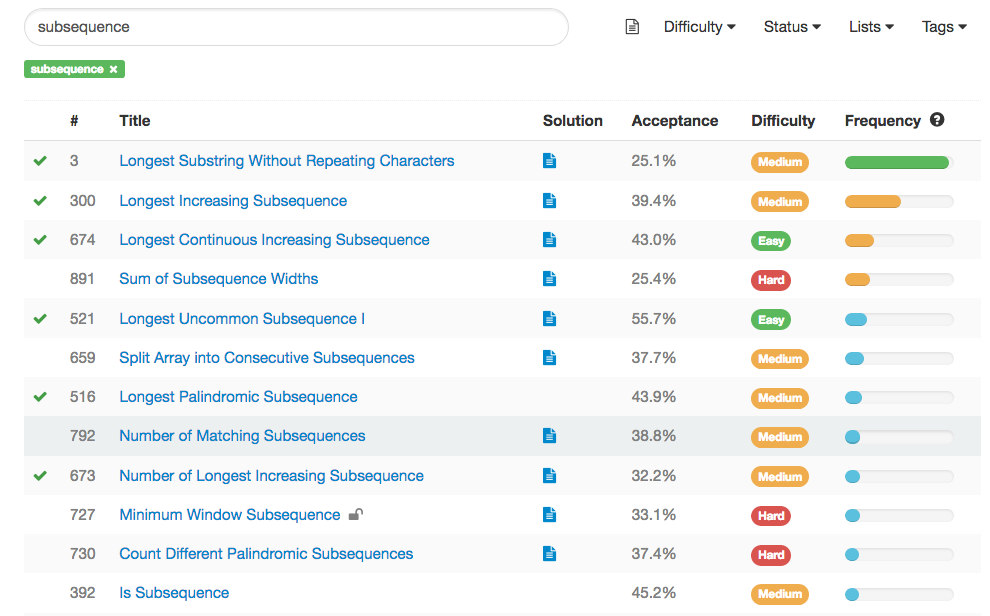
\includegraphics[width=0.8\columnwidth]{fig/subsequence_1.png}
    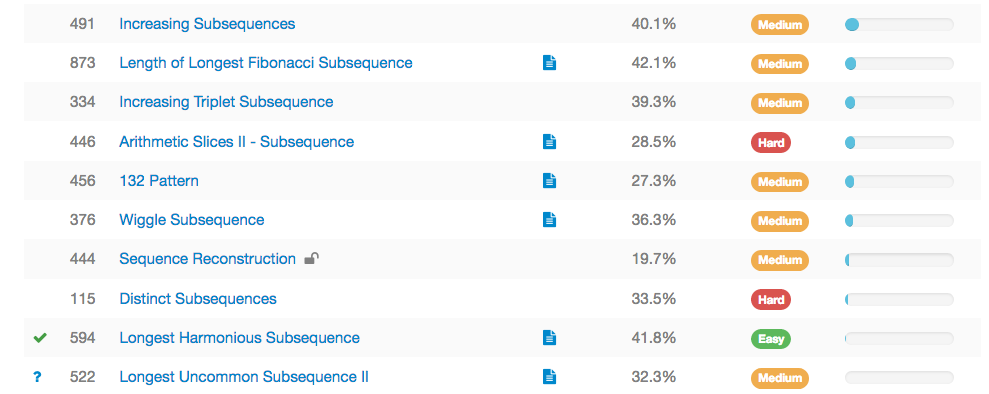
\includegraphics[width=0.8\columnwidth]{fig/subsequence_2.png}
    \caption{Subsequence Problems Listed on LeetCode}
    \label{fig:subsequence_problems}
\end{figure}

%%%%%%%%%%%%%%%%%%%%%%%%%%%%%%%%%%%%%%%%%%%%%%%%%%%%%%%%%%%%%%%%%%%%%%%%%%%
%%%%% Sum
%%%%%%%%%%%%%%%%%%%%%%%%%%%%%%%%%%%%%%%%%%%%%%%%%%%%%%%%%%%%%%%%%%%%%%%%%%%
\subsubsection{Sum}
In this section, to get sum we can choose to use hashmap to save the original list so that for the last element, we only check the hashmap, we can lower the complexity by one power of n. However, a better solution is to use two pointers or three pointers. for three pointers, the first one is to make sure the starting point. Also, we can think about divide and conquer.
\begin{lstlisting}
[-4,-1,-1,0,1,2]
i, l-> ``````<-r
\end{lstlisting}

\begin{enumerate}
    \item 15. 3Sum

Given an array S of n integers, are there elements a, b, c in S such that a + b + c = 0? Find all unique triplets in the array which gives the sum of zero.

Note: The solution set must not contain duplicate triplets.

For example, given array S = [-1, 0, 1, 2, -1, -4],
\begin{lstlisting}
A solution set is:
[
  [-1, 0, 1],
  [-1, -1, 2]
]
\end{lstlisting}

Solution: Should use three pointers, no extra space. i is the start point from [0,len-2], l,r is the other two pointers. l=i+1, r=len-1 at the beignning. The saving of time complexity is totally from the sorting algorithm.
\begin{lstlisting}
[-4,-1,-1,0,1,2]
i, l-> ``````<-r
\end{lstlisting}
How to delete repeat?
\begin{lstlisting}[language = Python]
def threeSum(self, nums):
    res = []
    nums.sort()
    for i in xrange(len(nums)-2):
        if i > 0 and nums[i] == nums[i-1]: #make sure pointer not repeat
            continue
        l, r = i+1, len(nums)-1
        while l < r:
            s = nums[i] + nums[l] + nums[r]
            if s < 0:
                l +=1 
            elif s > 0:
                r -= 1
            else:
                res.append((nums[i], nums[l], nums[r]))
                l+=1
                r-=1

                #after the first run, then check duplicate example.
                while l < r and nums[l] == nums[l-1]:
                    l += 1
                while l < r and nums[r] == nums[r+1]:
                    r -= 1
    return res
\end{lstlisting}
Use hashmap:
\begin{lstlisting}[language = Python]
def threeSum(self, nums):
        """
        :type nums: List[int]
        :rtype: List[List[int]]
        """
        res =[]
        nums=sorted(nums)
        if not nums:
            return []
        if nums[-1]<0 or nums[0]>0:
            return []
        end_position = len(nums)-2
        dic_nums={}
        for i in xrange(1,len(nums)):
            dic_nums[nums[i]]=i# same result save the last index
        
        for i in xrange(end_position):
            target = 0-nums[i]
            if i>0 and nums[i] == nums[i-1]: #this is to avoid repeat 
                continue
            if target<nums[i]: #if the target is smaller than this, we can not find them on the right side
                break
            for j in range(i+1,len(nums)): #this is to avoid repeat 
                if j>i+1 and nums[j]==nums[j-1]:
                    continue
                complement =target - nums[j]
                if complement<nums[j]: #if the left numbers are bigger than the complement, no need to keep searching
                    break
                if complement in dic_nums and dic_nums[complement]>j: #need to make sure the complement is bigger than nums[j]
                    res.append([nums[i],nums[j],complement])
        return res
\end{lstlisting}
The following code uses more time
\begin{lstlisting}[language = Python]
for i in xrange(len(nums)-2):
            if i > 0 and nums[i] == nums[i-1]:
                continue
            l, r = i+1, len(nums)-1
            while l < r:
                if l-1>=i+1 and nums[l] == nums[l-1]: #check the front
                    l += 1
                    continue
                if r+1<len(nums) and nums[r] == nums[r+1]:
                    r -= 1
                    continue
                s = nums[i] + nums[l] + nums[r]
                if s < 0:
                    l +=1 
                elif s > 0:
                    r -= 1
                else:
                    res.append((nums[i], nums[l], nums[r]))
                    l += 1; r -= 1
        return res
\end{lstlisting}

\item 18. 4Sum
\begin{lstlisting}[language = Python]
def fourSum(self, nums, target):
        def findNsum(nums, target, N, result, results):
            if len(nums) < N or N < 2 or target < nums[0]*N or target > nums[-1]*N:  # early termination
                return
            if N == 2: # two pointers solve sorted 2-sum problem
                l,r = 0,len(nums)-1
                while l < r:
                    s = nums[l] + nums[r]
                    if s == target:
                        results.append(result + [nums[l], nums[r]])
                        l += 1
                        r-=1
                        while l < r and nums[l] == nums[l-1]:
                            l += 1
                        while l < r and nums[r] == nums[r+1]:
                            r -= 1
                    elif s < target:
                        l += 1
                    else:
                        r -= 1
            else: # recursively reduce N
                for i in range(len(nums)-N+1):
                    if i == 0 or (i > 0 and nums[i-1] != nums[i]):
                        findNsum(nums[i+1:], target-nums[i], N-1, result+[nums[i]], results) #reduce nums size, reduce target, save result

results = []
        findNsum(sorted(nums), target, 4, [], results)
        return results
\end{lstlisting}

\item 454. 4Sum II

Given four lists A, B, C, D of integer values, compute how many tuples (i, j, k, l) there are such that A[i] + B[j] + C[k] + D[l] is zero.

To make problem a bit easier, all A, B, C, D have same length of N where $0 \leq N \leq 500$. All integers are in the range of -228 to 228–1 and the result is guaranteed to be at most 231–1.

Example:
\begin{lstlisting}
Input:
A = [ 1, 2]
B = [-2,-1]
C = [-1, 2]
D = [ 0, 2]

Output:
2
\end{lstlisting}

Explanation:

\begin{lstlisting}
The two tuples are:
1. (0, 0, 0, 1) -> A[0] + B[0] + C[0] + D[1] = 1 + (-2) + (-1) + 2 = 0
2. (1, 1, 0, 0) -> A[1] + B[1] + C[0] + D[0] = 2 + (-1) + (-1) + 0 = 0
\end{lstlisting}
Solution: if we use brute force, use 4 for loop, then it is $O(N^4)$. If we use divide and conquer, sum the first half, and save a dictionary (counter), time complexity is $O(2N^2)$. What if we have 6 sum, we can reduce it to $O(2N^3)$, what if 8 sum.

\begin{lstlisting}[language = Python]
def fourSumCount(self, A, B, C, D):
    AB = collections.Counter(a+b for a in A for b in B)
    return sum(AB[-c-d] for c in C for d in D)
\end{lstlisting}
\end{enumerate}
%%%%%%%%%%%%%%%%%%%%%%%%%%%%%%%%%%%%%%%%%%%%%%%%%%%%%%%%%%%%%%%%%%%%%%%%%%%
%%%%% Others
%%%%%%%%%%%%%%%%%%%%%%%%%%%%%%%%%%%%%%%%%%%%%%%%%%%%%%%%%%%%%%%%%%%%%%%%%%%
\subsubsection{Others}
For example, the following question would be used as follow up for question \textit{Longest Continuous Increasing Subsequence}

300. Longest Increasing Subsequence
\begin{lstlisting}
Given an unsorted array of integers, find the length of longest increasing subsequence.

For example,

 Given [10, 9, 2, 5, 3, 7, 101, 18],
 The longest increasing subsequence is [2, 3, 7, 101], therefore the length is 4. Note that there may be more than one LIS combination, it is only necessary for you to return the length.


Your algorithm should run in $O(n^2)$ complexity.

Follow up: Could you improve it to $O(nlogn)$ time complexity?
\begin{lstlisting}

Solution: Compared with the last question, this one loose the restriction that need to be continuous. For this problem, we need to understand it is not going to work with two pointers. It is not a brute-force $O(n^2)$ problem. It is a typical combination problem in recursive functions. So, at first, put the standard combination algorithm code here:
\begin{lstlisting}[language = Python]
def dfs(temp, idx):
            rslt.append(temp[:]) #pass temp[:] with shallow copy so that we wont change the result of rslt when temp is changed
            for i in range(idx, len(nums)):
                temp.append(nums[i])
                #backtrack
                dfs(temp, i+1)
                temp.pop()
                
                
        dfs([],0)
        return rslt
\end{lstlisting}

So, we use the backtracking-combination to enumerate all possible subsequence. The difference is here we do not unconditionally use this nums[i] in our result, only if nums[i]>tail, and the final length is the maximum of them all. $T(n) = max(T(n-1)+1, T(n-k)+1, …)$. So, the time complexity is $O(2^n)$. It passed 21/15 test cases with TLE. In this process, we transfer from the combination problem to dynamic programming.
\begin{lstlisting}[language = Python]
def lengthOfLIS(self, nums):
        """
        :type nums: List[int]
        :rtype: int
        """
        max_count = 0
        if not nums:
            return 0
        def backtrackingDFS(idx,tail):
            if idx==len(nums):
                
                return 0
            length = 0
            for i in range(idx,len(nums)):
                if nums[i]>tail:
                    length = max(1+backtrackingDFS(i+1, nums[i]), length)
            return length
        
        return backtrackingDFS(0,-maxsize)
\end{lstlisting}

Now, we know we are doing dynamic programming, if we already know the ans(idx), meaning the max length from somewhere, we do not need to do it again. With memoization: The time complexity is n subproblem, top-down recursive+memo.
\begin{lstlisting}[language = Python]
def lengthOfLIS(self, nums):
        """
        :type nums: List[int]
        :rtype: int
        """
        max_count = 0
        if not nums:
            return 0
        memo =[None for _ in range(len(nums))]
        def backtrackingDFS(idx,tail):
            if idx==len(nums):
                
                return 0
            if memo[idx]==None:
                length = 0
                for i in range(idx,len(nums)):
                    if nums[i]>tail:
                        length = max(1+backtrackingDFS(i+1, nums[i]), length)
                memo[idx]=length
            return memo[idx]
        
        return backtrackingDFS(0,-maxsize)
\end{lstlisting}

Now, we use dynamic programming which its solution can be found in Section~\ref{part2_sequence_dp}.  And bottom-up iterative. For [10,9,2,5,3], the length array is [1,1,1,2,2], for [4,10,4,3,8,9], we have [1, 2, 1, 1, 2, 3]. To find the rule, T(0)=1, idx, max(memo[i]),$0\leq i<idx$, $nums[idx]>nums[i]$. Now the time complexity is $O(n^2)$.

state: f[i] record the maximum length of increasing subsequence from 0-i.

function: f[i]: choose or not to choose

initialize: f[0]=1
\begin{lstlisting}[language = Python]
def lengthOfLIS(self, nums):
        """
        :type nums: List[int]
        :rtype: int
        """
        max_count = 0
        if not nums:
            return 0
        dp=[0 for _ in range(len(nums))]
        dp[0]=1
        maxans =1
        for idx in range(1,len(nums)): #current combine this to this subsequence, 10 to [], 9 to [10]
            pre_max=0
            for i in range(0,idx):
                if nums[idx]>nums[i]:
                    pre_max=max(pre_max, dp[i])
            dp[idx]=pre_max+1
            maxans=max(maxans,dp[idx])
            
        print(dp)
        return maxans
\end{lstlisting}

We can even speedup further by using binary search, the second loop we can use a binary search to make the time complexity $O(logn)$, and the dp array used to save the maximum ans. Each time we use binary search to find an insertion point, if it is at the end, then the length grow.
[4]->[4,10],->[4,10],[3,10],->[3,8]->[3,8,9]
\begin{lstlisting}[language = Python]
def lengthOfLIS(self, nums):
        """
        :type nums: List[int]
        :rtype: int
        """
        def binarySearch(arr,l,r,num):
            while l<r:
                mid = l+(r-l)//2
                if num>arr[mid]:
                    l=mid+1
                elif num<arr[mid]:
                    r=mid
                else:
                    return mid
            return l
        max_count = 0
        if not nums:
            return 0
        dp =[0 for _ in range(len(nums))]#save the maximum till now
        maxans =1
        length=0
        for idx in range(0,len(nums)): #current combine this to this subsequence, 10 to [], 9 to [10]
            pos = binarySearch(dp,0,length,nums[idx]) #find insertion point
            dp[pos]= nums[idx] #however if it is not at end, we replace it, current number
            if pos==length:
                length+=1
        print(dp)            
        return length
\end{lstlisting}

673. Number of Longest Increasing Subsequence

Given an unsorted array of integers, find the number of longest increasing subsequence.
\begin{lstlisting}
Example 1:

Input: [1,3,5,4,7]
Output: 2
Explanation: The two longest increasing subsequence are [1, 3, 4, 7] and [1, 3, 5, 7].

Example 2:
Input: [2,2,2,2,2]
Output: 5
Explanation: The length of longest continuous increasing subsequence is 1, and there are 5 subsequences' length is 1, so output 5.
\textit{Note: Length of the given array will be not exceed 2000 and the answer is guaranteed to be fit in 32-bit signed int.}
\end{lstlisting}

Solution: Another different problem, to count the number of the max subsequence. Typical dp:

state: f[i]
\begin{lstlisting}[language = Python]
from sys import maxsize
class Solution:
    def findNumberOfLIS(self, nums):
        """
        :type nums: List[int]
        :rtype: int
        """
        max_count = 0
        if not nums:
            return 0
        memo =[None for _ in range(len(nums))]
        rlst=[]
        def recursive(idx,tail,res):
            if idx==len(nums):
                rlst.append(res)
                return 0
            if memo[idx]==None:
                length = 0
                if nums[idx]>tail:
                    addLen = 1+recursive(idx+1, nums[idx],res+[nums[idx]])
                    notAddLen = recursive(idx+1, tail,res)
                    return max(addLen,notAddLen)
                else:
                    return recursive(idx+1, tail,res)
        
        
        ans=recursive(0,-maxsize,[])
        count=0
        for lst in rlst:
            if len(lst)==ans:
                count+=1
                
        return count
\end{lstlisting}

Using dynamic programming, the difference is we add a count array.
\begin{lstlisting}[language = Python]
from sys import maxsize
class Solution:
    def findNumberOfLIS(self, nums):
        N = len(nums)
        if N <= 1: return N
        lengths = [0] * N #lengths[i] = longest ending in nums[i]
        counts = [1] * N #count[i] = number of longest ending in nums[i]

    for idx, num in enumerate(nums): #i
            for i in range(idx): #j
                if nums[i] < nums[idx]: #bigger 
                    if lengths[i] >= lengths[idx]:
                        lengths[idx] = 1 + lengths[i] #set the biggest length
                        counts[idx] = counts[i] #change the count
                    elif lengths[i] + 1 == lengths[idx]: #if it is a tie
                        counts[idx] += counts[i] #increase the current count by count[i]

longest = max(lengths)
        print(counts)
        print(lengths)
        return sum(c for i, c in enumerate(counts) if lengths[i] == longest)
\end{lstlisting}

128. Longest Consecutive Sequence
\begin{lstlisting}
Given an unsorted array of integers, find the length of the longest consecutive elements sequence.

For example,
 Given [100, 4, 200, 1, 3, 2],
 The longest consecutive elements sequence is [1, 2, 3, 4]. Return its length: 4.
 
 Your algorithm should run in O(n) complexity.
 \end{lstlisting}

Solution: Not thinking about the O(n) complexity, we can use sorting to get [1,2,3,4,100,200], and then use two pointers to get [1,2,3,4].

How about O(n)? We can pop out a number in the list, example, 4 , then we use while first-1 to get any number that is on the left side of 4, here it is 3, 2, 1, and use another to find all the bigger one and remove these numbers from the nums array.
\begin{lstlisting}[language =Python]
def longestConsecutive(self, nums):
        nums = set(nums)
        maxlen = 0
        while nums:
            first = last = nums.pop()
            while first - 1 in nums: #keep finding the smaller one
                first -= 1
                nums.remove(first)
            while last + 1 in nums: #keep finding the larger one
                last += 1
                nums.remove(last)
            maxlen = max(maxlen, last - first + 1)
        return maxlen
\end{lstlisting}


%%%%%%%%%%%%%%%%%%%%%%%%%%%%%%%%%%%%%%%%%%%%%%%%%%%%%%%%%%%%%%%%%%%%%%%%%%%
%%%%% Merge List
%%%%%%%%%%%%%%%%%%%%%%%%%%%%%%%%%%%%%%%%%%%%%%%%%%%%%%%%%%%%%%%%%%%%%%%%%%%
\subsection{Merge and Partition}
\subsubsection{Merge Lists}
We can use divide and conquer (see the merge sort) and the priority queue.
\subsubsection{Partition Lists}
%%%%%%%%%%%%%%%%%%%%%%%%%%%%%%%%%%%%%%%%%%%%%%%%%%%%%%%%%%%%%%%%%%%%%%%%%%%
%%%%% Intersection
%%%%%%%%%%%%%%%%%%%%%%%%%%%%%%%%%%%%%%%%%%%%%%%%%%%%%%%%%%%%%%%%%%%%%%%%%%%
\subsection{Intersection}
For problems to get intersections of lists, we can use hashmap, which takes $O(m+n)$ time complexity. Also, we can use sorting at first and use two pointers one start from the start of each array. Examples are shown as below;
\begin{enumerate}
    \item  349. Intersection of Two Arrays (Easy)
    
     Given two arrays, write a function to compute their intersection.

Example:
\begin{lstlisting}
Given nums1 = [1, 2, 2, 1], nums2 = [2, 2], return [2].
\end{lstlisting}

Note:
\begin{itemize}
    \item Each element in the result must be unique.
    \item The result can be in any order.
\end{itemize}
Solution 1: Using hashmap, here we use set to convert, this takes 43ms. 
\begin{lstlisting}[language = Python]
def intersection(self, nums1, nums2):
    """
    :type nums1: List[int]
    :type nums2: List[int]
    :rtype: List[int]
    """
    if not nums1 or not nums2:
        return []
    if len(nums1) > len(nums2):
        nums1, nums2 = nums2, nums1
    ans = set()
    nums1 = set(nums1)
    for e in nums2:
        if e in nums1:
            ans.add(e)
    return list(ans)
\end{lstlisting}
Solution2: sorting at first, and then use pointers. Take 46 ms. 
\begin{lstlisting}[language = Python]
def intersection(self, nums1, nums2):
    """
    :type nums1: List[int]
    :type nums2: List[int]
    :rtype: List[int]
    """
    nums1.sort()
    nums2.sort()
    r = set()
    i, j = 0, 0
    while i < len(nums1) and j < len(nums2):
        if nums1[i] < nums2[j]:
            i += 1
        elif nums1[i] > nums2[j]:
            j += 1
        else:
            r.add(nums1[i])
            i += 1
            j += 1
    return list(r)
\end{lstlisting}
\item 350. Intersection of Two Arrays II(Easy)

 Given two arrays, write a function to compute their intersection.

Example:
\begin{lstlisting}
Given nums1 = [1, 2, 2, 1], nums2 = [2, 2], return [2, 2].
\end{lstlisting}

Note:
\begin{itemize}
    \item Each element in the result should appear as many times as it shows in both arrays.
    \item The result can be in any order.
\end{itemize}

Follow up:
\begin{enumerate}
    \item  What if the given array is already sorted? How would you optimize your algorithm?
    \item What if nums1's size is small compared to nums2's size? Which algorithm is better?
    \item What if elements of nums2 are stored on disk, and the memory is limited such that you cannot load all elements into the memory at once?
\end{enumerate}

\end{enumerate}
%%%%%%%%%%%%%%%%%%%%%%%%%%%%%%%%%%%%%%%%%%%%%%%%%%%%%%%%%%%%%%%%%%%%%%%%%%%
%%%%% Exercises
%%%%%%%%%%%%%%%%%%%%%%%%%%%%%%%%%%%%%%%%%%%%%%%%%%%%%%%%%%%%%%%%%%%%%%%%%%%
\section{Exercises}
%%%%%%%%%%%%%%%%%%%%%%%%%%%%%%%%%%%%%%%%%%%%%%%%%%%%%%%%%%%%%%%%%%%%%%%%%%%
%%%%% Subarray
%%%%%%%%%%%%%%%%%%%%%%%%%%%%%%%%%%%%%%%%%%%%%%%%%%%%%%%%%%%%%%%%%%%%%%%%%%%
\subsection{Subarray}
\subsubsection{Absolute-conditioned Subarray}
\begin{enumerate}
    \item 930. Binary Subarrays With Sum
    \begin{lstlisting}
    In an array A of 0s and 1s, how many non-empty subarrays have sum S?
Example 1:

Input: A = [1,0,1,0,1], S = 2
Output: 4
Explanation: 
The 4 subarrays are bolded below:
[1,0,1,0,1]
[1,0,1,0,1]
[1,0,1,0,1]
[1,0,1,0,1]
Note:

    A.length <= 30000
    0 <= S <= A.length
    A[i] is either 0 or 1.
\end{lstlisting}
Answer: this is exactly the third time of maximum subarray, the maximum length of subarry with a certain value. We solve it using prefix sum and a hashmap to save the count of each value. 
\begin{lstlisting}[language=Python]
import collections
class Solution:
    def numSubarraysWithSum(self, A, S):
        """
        :type A: List[int]
        :type S: int
        :rtype: int
        """
        dict = collections.defaultdict(int) #the value is the number of the sum occurs
        dict[0]=1 #prefix sum starts from 0 and the number is 1
        prefix_sum, count=0, 0
        for v in A:
            prefix_sum += v
            count += dict[prefix_sum-S] # increase the counter of the appearing value k, default is 0
            dict[prefix_sum] += 1 # update the count of prefix sum, if it is first time, the default value is 0
        return count
\end{lstlisting}
We can write it as:
\begin{lstlisting}[language=Python]
    def numSubarraysWithSum(self, A, S):
        """
        :type A: List[int]
        :type S: int
        :rtype: int
        """
        P = [0]
        for x in A: P.append(P[-1] + x)
        count = collections.Counter()

        ans = 0
        for x in P:
            ans += count[x]
            count[x + S] += 1

        return ans
\end{lstlisting}
Also, it can be solved used a modified sliding window algorithm. For sliding window, we have $i,j$ starts from 0, which represents the window. Each iteration j will move one position. For a normal sliding window, only if the sum is larger than the value, then we shrink the window size by one. However, in this case, like in the example $1, 0, 1, 0, 1$, when $j = 5$, $i = 1$, the sum is $2$, but the algorithm would miss the case of $i = 2$, which has the same sum value. To solve this problem, we keep another index $i_hi$, in addition to the moving rule of $i$, it also moves if the sum is satisfied and that value is $0$. This is actually a Three pointer algorithm. 
\begin{lstlisting}[language=Python]
    def numSubarraysWithSum(self, A, S):
        i_lo, i_hi, j = 0, 0, 0 #i_lo <= j
        sum_lo = sum_hi = 0
        ans = 0
        while j < len(A):
            # Maintain i_lo, sum_lo:
            # While the sum is too big, i_lo += 1
            sum_lo += A[j]
            while i_lo < j and sum_lo > S:
                sum_lo -= A[i_lo]
                i_lo += 1

            # Maintain i_hi, sum_hi:
            # While the sum is too big, or equal and we can move, i_hi += 1
            sum_hi += A[j]
            while i_hi < j and (
                    sum_hi > S or sum_hi == S and not A[i_hi]):
                sum_hi -= A[i_hi]
                i_hi += 1

            if sum_lo == S:
                ans += i_hi - i_lo + 1
            j += 1

        return ans
\end{lstlisting}
\item 523. Continuous Subarray Sum
\begin{lstlisting}
Given a list of non-negative numbers and a target integer k, write a function to check if the array has a continuous subarray of size at least 2 that sums up to the multiple of k, that is, sums up to n*k where n is also an integer.

Example 1:
Input: [23, 2, 4, 6, 7],  k=6
Output: True
Explanation: Because [2, 4] is a continuous subarray of size 2 and sums up to 6.

Example 2:
Input: [23, 2, 6, 4, 7],  k=6
Output: True
Explanation: Because [23, 2, 6, 4, 7] is an continuous subarray of size 5 and sums up to 42.

Note:
The length of the array won't exceed 10,000.
You may assume the sum of all the numbers is in the range of a signed 32-bit integer.
\end{lstlisting}
Answer: This is a mutant of the subarray with value k. The difference here, we save the prefix sum as the reminder of k. if $(a+b)\%k=0$, then $(a\%k+b\%k)/k=1$.
\begin{lstlisting}[language=Python]
class Solution:
    def checkSubarraySum(self, nums, k):
        """
        :type nums: List[int]
        :type k: int
        :rtype: bool
        """
        
        if not nums:
            return False
        k = abs(k)
        prefixSum = 0
        dict = collections.defaultdict(int)
        dict[0]=-1
        for i, v in enumerate(nums):
            prefixSum += v
            if k!=0:
                prefixSum %= k
            if prefixSum in dict and (i-dict[prefixSum])>=2:
                    return True
            if prefixSum not in dict:
                dict[prefixSum] = i
        return False
\end{lstlisting}
\end{enumerate}
\subsubsection{Vague-conditioned Subarray}

%%%%%%%%%%%%%%%%%%%%%%%%%%%%%%%%%%%%%%%%%%%%%%%%%%%%%%%%%%%%%%%%%%%%%%%%%%%
%%%%% Subsequence
%%%%%%%%%%%%%%%%%%%%%%%%%%%%%%%%%%%%%%%%%%%%%%%%%%%%%%%%%%%%%%%%%%%%%%%%%%%
\subsection{Subsequence}
\begin{enumerate}
    \item 594. Longest Harmonious Subsequence

We define a harmonious array is an array where the difference between its maximum value and its minimum value is exactly 1.

Now, given an integer array, you need to find the length of its longest harmonious subsequence among all its possible subsequences.

Example 1:
\begin{lstlisting}
Input: [1,3,2,2,5,2,3,7]
Output: 5
Explanation: The longest harmonious subsequence is [3,2,2,2,3].
\end{lstlisting}

\textit{Note: The length of the input array will not exceed 20,000.}

Solution: at first, use a Counter to save the whole set. Then visit the counter dictionary, to check key+1 and key-1, only when the item is not zero, we can count it as validate, or else it is 0.
\begin{lstlisting}[language = Python]
from collections import Counter
class Solution:
    def findLHS(self, nums):
        """
        :type nums: List[int]
        :rtype: int
        """
        if not nums or len(nums)<2:
            return 0
        count=Counter(nums) #the list is sorted by the key value
        maxLen = 0
        for key,item in count.items(): #to visit the key: item in the counter
            if count[key+1]: #because the list is sorted, so we only need to check key+1
                maxLen = max(maxLen,item+count[key+1])
            
            # if count[key-1]:
            #     maxLen=max(maxLen, item+count[key-1])
        return maxLen
\end{lstlisting}

\item 521. Longest Uncommon Subsequence I

Given a group of two strings, you need to find the longest uncommon subsequence of this group of two strings. The longest uncommon subsequence is defined as the longest subsequence of one of these strings and this subsequence should not be any subsequence of the other strings.

A subsequence is a sequence that can be derived from one sequence by deleting some characters without changing the order of the remaining elements. Trivially, any string is a subsequence of itself and an empty string is a subsequence of any string.

The input will be two strings, and the output needs to be the length of the longest uncommon subsequence. If the longest uncommon subsequence doesn’t exist, return -1.

Example 1:
\begin{lstlisting}
Input: "aba", "cdc"
Output: 3
Explanation: The longest uncommon subsequence is "aba" (or "cdc"), 
because "aba" is a subsequence of "aba", 
but not a subsequence of any other strings in the group of two strings.
\end{lstlisting}

\textit{Note:}

    \textit{Both strings’ lengths will not exceed 100.}
    
    \textit{Only letters from a ~ z will appear in input strings.}

Solution: if we get more examples, we could found the following rules, “aba”,”aba” return -1,
\begin{lstlisting}[language = Python]
def findLUSlength(self, a, b):
        """
        :type a: str
        :type b: str
        :rtype: int
        """
        if len(b)!=len(a):
            return max(len(a),len(b))
        #length is the same
        return len(a) if a!=b else -1
\end{lstlisting}
\item 424. Longest Repeating Character Replacement

Given a string that consists of only uppercase English letters, you can replace any letter in the string with another letter at most k times. Find the length of a longest substring containing all repeating letters you can get after performing the above operations.

\textit{Note:}

 \textit{Both the string’s length and k will not exceed 104.}

Example 1:
\begin{lstlisting}
Input:
s = "ABAB", k = 2

Output:
4
\end{lstlisting}

Explanation:
Replace the two 'A's with two 'B's or vice versa.

Example 2:
\begin{lstlisting}
Input:
s = "AABABBA", k = 1

Output:
4
\end{lstlisting}

Explanation:
Replace the one 'A' in the middle with 'B' and form "AABBBBA".
The substring "BBBB" has the longest repeating letters, which is 4.

Solution: the brute-force recursive solution for this, is try to replace any char into another when it is not equal or choose not too. LTE
\begin{lstlisting}[language = Python]
#brute force, use recursive function to write brute force solution
        def replace(news, idx, re_char, k):
            nonlocal maxLen
            if k==0 or idx==len(s):
                maxLen = max(maxLen, getLen(news))
                return

if s[idx]!=re_char: #replace
                news_copy=news[:idx]+re_char+news[idx+1:]
                replace(news_copy, idx+1, re_char, k-1)
            replace(news[:], idx+1, re_char,k)
        
        #what if we only have one char
        # for char1 in chars.keys():
        #     replace(s[:],0,char1, k)
\end{lstlisting}
To get the BCR, think about the sliding window. The longest repeating string we can by number of replacement = `length of string max(numer of occurence of letter i), i=’A’ to ‘Z’. With the constraint, which means the equation needs to be $\leq k$. So we can use sliding window to record the max occurence, and when the constraint is violated, we shrink the window. Given an example, strs= “BBCABBBAB”, k=2, when i=0, and j=7, 8–5=3>2, which is at A, we need to shrink it, the maxCharCount changed to 4, i=1, so that 8–1–4=3, i=2, 8–2–3=3, 8–3–3=2, so i=3, current length is 5.
\begin{lstlisting}[language = Python]
def characterReplacement(self, s, k):
        """
        :type s: str
        :type k: int
        :rtype: int
        """
        i,j = 0,0 #sliding window
        counter=[0]*26
        ans = 0
        maxCharCount = 0
        while j<len(s):
            counter[ord(s[j])-ord('A')]+=1
            maxCharCount = max(maxCharCount, counter[ord(s[j])-ord('A')])
            while j-i+1-maxCharCount>k: #now shrink the window
                counter[ord(s[i])-ord('A')]-=1
                i+=1
                #updata max
                maxCharCount=max(counter)
            ans=max(ans, j-i+1)
            j+=1
                
        return ans
\end{lstlisting}

\item 395. Longest Substring with At Least K Repeating Characters

Find the length of the longest substring T of a given string (consists of lowercase letters only) such that every character in T appears no less than k times.

Example 1:
\begin{lstlisting}
Input:
s = "aaabb", k = 3

Output:
3
\end{lstlisting}

The longest substring is "aaa", as 'a' is repeated 3 times.

Example 2:
\begin{lstlisting}
Input:
s = "ababbc", k = 2

Output:
5
\end{lstlisting}

The longest substring is "ababb", as 'a' is repeated 2 times and 'b' is repeated 3 times.

Solution: use dynamic programming with memo: Cons: it takes too much space, and with LTE.
\begin{lstlisting}[language = Python]
from collections import Counter, defaultdict
class Solution:
    def longestSubstring(self, s, k):
        """
        :type s: str
        :type k: int
        :rtype: int
        """
        if not s:
            return 0
        if len(s)<k:
            return 0
        count = Counter(char for char in s)
        print(count)
        memo=[[None for col in range(len(s))] for row in range(len(s))]

def cut(start,end,count):
            if start>end:
                return 0
            if memo[start][end]==None:
                if any(0<item<k for key,item in count.items()):
                    newCounterF=count.copy()
                    newCounterF[s[start]]-=1
                    newCounterB=count.copy()
                    newCounterB[s[end]]-=1
                    #print(newsF,newsB)
                    memo[start][end]= max(cut(start+1, end, newCounterF), cut(start, end-1, newCounterB))
                else:
                    memo[start][end] = end-start+1
            return memo[start][end]
        return cut(0,len(s)-1,count)
\end{lstlisting}

Now, use sliding window, we use a pointer mid, what start from 0, if the whole string satisfy the condition, return len(s). Otherwise, use two while loop to separate the string into three substrings: left, mid, right. left satisfy, mid unsatisfy, right unknown.
\begin{lstlisting}[language = Python]
from collections import Counter, defaultdict
class Solution:
    def longestSubstring(self, s, k):
        """
        :type s: str
        :type k: int
        :rtype: int
        """
        if not s:
            return 0
        if len(s)<k:
            return 0
        count = Counter(char for char in s)
        mid=0 #on the left side, from 0-mid, satisfied elments
        while mid<len(s) and count[s[mid]]>=k:
            mid+=1
        if mid==len(s): return len(s) 
        left = self.longestSubstring(s[:mid],k) #"ababb"
        #from pre_mid - cur_mid, get rid of those cant satisfy the condition
        while mid<len(s) and count[s[mid]]<k:
            mid+=1
        #now the right side keep doing it
        right = self.longestSubstring(s[mid:],k)
        return max(left,right)
\end{lstlisting}

\subsection{Intersection}
\item 160. Intersection of Two Linked Lists (Easy)

Write a program to find the node at which the intersection of two singly linked lists begins.

For example, the following two linked lists:
\begin{lstlisting}

        
A:          a1 -> a2
                  \
                     c1 -> c2 -> c3
                  /            
B:     b1 -> b2 -> b3
\end{lstlisting}

begin to intersect at node c1.

Notes:
\begin{itemize}
    \item If the two linked lists have no intersection at all, return null.
    \item The linked lists must retain their original structure after the function returns.
    \item You may assume there are no cycles anywhere in the entire linked structure.
    \item Your code should preferably run in O(n) time and use only O(1) memory.
\end{itemize}


\end{enumerate}
\end{document}